\minitoc  % Affiche la table des matières pour ce chapitre

% ==================================================================================================================================
% Intégrale d'une fonction

\section{Intégrale d'une fonction}

\subsection{Fonction étagée et fonction intégrale}

\begin{definition}[Intégrale d'une fonction étagée]
    Soit $e$ une fonction étagée positive. On a $e = \sum_{i=1}^{n} \lambda_i 1_{A_i}$ où $A_i = e^{-1}(\{\lambda_i\})$ où $\lambda_i \in \R_+$.
    L'intégrale de $e$ par rapport à $\mu$ est de la forme :
        \[ \boxed{ \int e \; d \mu = \sum_{i=1}^{n} \lambda_i \mu (A_i) } \] 
\end{definition}

\begin{definition}[Fonction intégrale]
    Soit $f \in \overline{\mathcal{M}_+}(X)$, alors : 
        \[ \int f \; d \mu := \sup \Bigl( \Bigr\{ \int e \; d \mu : e \text{ fonction étagée positive tq } e \leq f \Bigl\}) \Bigr) \] 
    Ainsi, l'intégrale d'une fonction mesurable positive existe toujours.
    On peut donc définir la fonction intégrale telle que :
        \[ \int . \; d \mu : 
            \begin{cases}
                \overline{\mathcal{M}_+}(X) & \longrightarrow \overline{\R_+} \\ 
                f & \longmapsto \int f \; d \mu 
            \end{cases}
        \] 
\end{definition}

\begin{prop}(Propriétés de l'intégrale)
    La fonction intégrale vérifie les propriétés suivantes :
    \begin{itemize}
        \item \underline{Extension de la mesure :} $\forall A \in \mathcal{B}, \int 1 _A \; d \mu = \mu(A)$ 
        \item \underline{Linéarité positive :} $\forall f, g \in \overline{\mathcal{M}_+}(X), \forall \alpha \in \R_+$ on a :
            \[ \int (f + \alpha g) \; d \mu = \int f \; d \mu + \alpha \int g \; d \mu \]
        \item \underline{Convergence Monotone :} Pour toute suite croissante de fonctions mesurables positives (étendues) $(f_n)$, on a :
            \[ \boxed { \int \lim_{n\to\infty} f_n \; d \mu = \lim_{n\to\infty} \int f_n \; d \mu }\] 
    \end{itemize}
\end{prop}

\subsection{Intégrabilité (fonction positive)}

\begin{definition}[Fonction Intégrable (Cas Réel Positif)]
    Une fonction $f \in \overline{\mathcal{M}_+}(X)$ est dite intégrable si $\int f \;d \mu < \infty $.
\end{definition}

\begin{remark}
    Quelques remarques concernant la notation... 
    \begin{itemize}
        \item $\overline{\mathcal{L}_+^1}(X)$ est l'ensemble des fonctions $f : X \rightarrow \overline{\R_+}$ intégrables.
        \item ${\mathcal{L}_+^1}(X)$ est l'ensemble des fonctions intégrables de $X$ vers $\R_+$ mais non étendues.
        \item On remarquera que intégrable implique mesurable. La réciproques est généralement fause.
    \end{itemize}
\end{remark}

\begin{prop}[Croissance de l'intégrale]
    La fonction intégrale est croissante.
    \[ \text{i.e } \forall f,g \in \overline{\mathcal{M}_+}(X) \text{ si } f \leq g, \quad \text{alors } \int f \; d \mu \leq \int g \; d \mu \] 
\end{prop}

\begin{quote}
    \footnotesize 
    \begin{proof}
        Soient $f, g \in \overline{\mathcal{M}_+}(X)$ telles que $f \leq g$ alors $g = g-f+f$ où $g-f \geq 0 $ \\
        D'où : $ \int g \; d \mu = \int (g-f) \; d \mu + \int f \; d \mu \geq \int f \; d \mu $
    \end{proof}
    \normalsize
\end{quote}

\begin{remark}
    Pour tout $f,g \in \overline{\mathcal{M}_+}(X)$ telles que $f \leq g$ si $g$ est intégrable alors $f \in \overline{\mathcal{L}_+^1}(X)$.
\end{remark}

\subsection{Intégrabilité (fonction à valeurs complexes)}

\begin{definition}[Fonction Intégrable]
    Soit $f \in \mathcal{M}(x)$ une fonction mesurable d'un ensemble $X$ vers $\C$. 
    On dit que $f$ est intégrable si la fonction $|f| \in \mathcal{M}_+(X)$ est intégrable (ici on parle du module). \\
    On notera $\mathcal{L}^1(X)$ l'ensemble des fonction intégrables de $X$ vers $\C$.
\end{definition}

\newpage
\begin{definition}[Intégrale d'une fonction à valeurs complexes]
    Soit $f \in \mathcal{L}^1(X)$, distinguons deux cas :
    \begin{itemize}
        \item \textbf{Cas réel positif :} si $f \in \mathcal{L}^1_\R(X)$ alors soient :
            \begin{align*}
                f_+ : x \longmapsto \max (0, f(x)) \\ 
                f_+ = \sup (0, f) \\ 
                f_- : x \longmapsto \min (0, f) \\
                f_- = - \inf (0, f)
            \end{align*}
            on pose alors :
                \[ \int f \; d \mu = \int f_+ \; d \mu - \int f_- \; d \mu \] 
        \item \textbf{Cas complexe :} si $f \in \mathcal{L}^1(X)$ on pose :
            \[ \int f \; d \mu = \int \Re f \; d \mu - i \int \Im f \; d \mu \]
    \end{itemize}
\end{definition}

\begin{prop}[Propriétés de l'intégrale...2]
    Quelques propriétés sur l'intégrale...
    \begin{enumerate}
        \item \textbf{Linéarité :} La fonction intégrale sur $\mathcal{L}^1(X)$ est linéaire et $\mathcal{L}^1(X)$ est un sev de $\C$.
        \item \textbf{Croissance}
        \item \textbf{Majoration par le module :} si $f \in \mathcal{L}^1(X)$ alors $\Big| \int f \; d \mu \Big| \leq \int |f| \; d \mu$
    \end{enumerate}
\end{prop}

\begin{theorem}[Critère d'intégrabilité des fonctions bornées]
    Si $(X,\mathcal{B},\mu)$ est un espace mesuré \textbf{fini} alors toutes fonction $ f \in \mathcal{M}(X)$ \textbf{bornée} est intégrable. 
\end{theorem}

\subsection{Extension par zéro et intégrale restreinte}

\begin{definition}[Fonction extension par zéro]
    Soit $f : A \rightarrow \C$ où $A \subset X$, alors l'extension par zéro de $f$ est la fonction :
        \[ e_X(f) : 
            \begin{cases}
                X \longrightarrow \C \\
                x \longmapsto \begin{cases}
                                    f(x) \text{ si } x \in A \\
                                    0 \text{ sinon }
                                \end{cases}
            \end{cases} \] 
\end{definition}

\begin{definition}[Intégrale restreinte]
    Une fonction $f$ intégrable sur $X$ positive (resp. à valeurs complexes) est dite intégrable sur $A \subset X$ si la restriction de $f$ (resp. la restriction $|f|$) à $A$ est intégrable.
\end{definition}

\newpage 

\begin{prop}[Intégrale restreinte]
    Soient $g \in \overline{\mathcal{M}_+(A)}, A \subset X$ et $e_x$ son extension par zéro sur $X$.
    Soit $1_A$ la fonction indicatrice de $A$.
    \begin{itemize}
        \item \textbf{Intégrale et extension par zéro :}
            \[ \int_{X} e_x(g) \; d \mu = \int_{A} g \; d \mu \] 
            $g$ est donc intégrable sur A si $e_x(g)$ est intégrable sur $X$.
        \item \textbf{Intégrale restreinte et indicatrice :}
            \begin{itemize}
                \item si $f \in \mathcal{M}_+(X)$ alors $\int_{A} f \; d \mu = \int_{X} f \times 1_A \; d \mu $ 
                \item si $f \in \mathcal{M}(X)$ alors $f$ est intégrable sur $A$ si $f \times 1_A$ est intégrable sur $X$ et dans ce cas :
                    \[ \boxed{ \int_{A} f \; d \mu = \int_{X} f \times 1_A \; d \mu } \] 
            \end{itemize}
        \item \textbf{Intégrabilité et restriction :} soit $f \in \mathcal{L}^1(X)$ alors $f\restriction_A \in \mathcal{L}^1(X)$ où $A \subset X$ et 
                \[ \int_A |f| \; d \mu \leq \in_X |f| \; d \mu \]
        \item \textbf{Relation de Chasles généralisée :} Soit $(A_n)_{n\in\N}$ une suite de parties 
            mesurables deux à deux disjointes et soit $f \in \overline{\mathcal{M}_+(X)}$ alors: 
                \[ \int_{\bigcup_{n \in \N} A_n} f \; d \mu = \sum_{n=0}^{\infty} \int_{A_n} f \; d \mu \]
            Pour le cas complexe, si $f \in \overline{\mathcal{M}(X)}$  alors $f$ est intégrable sur $(A_n)_{n\in\N}$ 
            ssi $$\sum_{n=0}^{\infty} \int_{A_n} |f| \; d \mu \le \infty $$
            et dans ce cas on a l'égalité (dans $\C$) :
                \[ \int_{\bigcup_{n \in \N} A_n} f \; d \mu = \sum_{n=0}^{\infty} \int_{A_n} f \; d \mu \]
        \item \textbf{Indivisibilité des parties négligeables :} Si $N$ est une partie négligeable, toute fonction mesurable est intégrable sur $N$ et son intégrale est nulle.
                \[ \text{i.e } \int_N f \; d \mu = 0 \]
    \end{itemize}
\end{prop}
\newpage

\subsection{Intervalles non compacts et rappels}
\begin{theorem}[Intégration sur un intervalle \textbf{non compact}]
    \begin{enumerate}
        \item \textbf{Cas positif :} Soit $f \in \overline{\mathcal{M}_+([a,c[)}$ on a 
        \[ \boxed{ \int_{[a,c[} f \; d \lambda = \underset{b \in [a,c[}{\sup} \int_{[a,c[} f \; d \lambda} \]
        en particulier $ f \in \mathcal{L}^1_+([a,c[)$ :
        \begin{itemize}
            \item[\underline{ssi}] $\Bigl\{ \int_{[a,b]} f \; d \lambda : b \in [a,c[ \Bigr\}$ est majoré dans $\R_+$ 
            \item[\underline{ssi}] il existe une suite $(b_n)$ croissante de $[a,c[$ qui tend vers $c$ telle que $ (\int_{[a,bn]} f \; d \lambda)_n$ est majorée.
        \end{itemize}
        \item \textbf{Cas non positif :} Soit $ f \in \mathcal{L}^1([a,c[)$ à valeurs complexes alors :
            \[ \boxed{ \lim_{b \to c} \int_{[a,b]} d \; \lambda = \int_{[a,c[} f \; d \lambda} \] 
    \end{enumerate}
\end{theorem}

\textbf{Exemple :}

\begin{minipage}{0.4\textwidth}  % Largeur du graphique
    \begin{tikzpicture}
      \begin{axis}[
          domain=0.1:10,
          samples=200,
          width=\linewidth,  % Adapte la largeur au minipage
          height=4cm,
          xlabel=$x$,
          ylabel=$f(x)$,
          axis lines=middle,
          % xtick={0,2,4,6,8,10},
          % ytick={0,0.5,1},
          ymin=-0.5, ymax=1.5,
          % title={$f(x) = \frac{\sin(x)}{x}$ pour $x > 0$ et $f(0) = 1$},
          every axis plot/.append style={black, thick}
        ]

        % Définition des chemins pour la courbe et l'axe des abscisses
        \addplot[name path=curve, domain=0.1:10, black, thick] {sin(deg(x))/x};
        \addplot[name path=axis, domain=0.1:10] {0};

        % Zone hachurée entre la courbe et l'axe des abscisses
        \addplot [
          fill=gray, % Couleur de hachure
          opacity=0.3
        ]
        fill between [
          of=curve and axis, % Remplissage entre la courbe et l'axe des abscisses
        ];

        % Point en (0, 1) pour x = 0
        \addplot[only marks, mark=*] coordinates {(0,1)};

      \end{axis}
    \end{tikzpicture}
\end{minipage}%
\hfill
\begin{minipage}{0.55\textwidth}  % Largeur pour le texte
    $f : [a,c[ \longrightarrow \C$ peut avoir une intégrale impropre convergente sans nécessairement être intégrable au sens de Lebesque. 
    Par exemple la fonction ci-contre n'a pas d'intégrale définie au sens de Lebesgues mais au sens de Riemann oui.
    \[
    f(x) = \frac{\sin(x)}{x} \text{ lorsque } x > 0, \quad f(0) = 1.
    \]
\end{minipage}


\begin{example}[Intégrale de Riemann]
    \[ f_\alpha :
        \begin{cases}
            \R_+^* \longrightarrow \R \\
            t \longmapsto \frac{1}{t^\alpha}, \alpha \ge 0
        \end{cases}
    \] 
    \begin{enumerate}
        \item sur $[1, \infty[, f_\alpha$ est intégrable ssi $\alpha \ge 1$
        \item sur $]0, 1[, f_\alpha$ est intégrable ssi $\alpha \le 1$
    \end{enumerate}
\end{example}

\begin{example}[Intégrales de Bertrand]
    \[ f_{\alpha, \beta} :
        \begin{cases}
            \R_+^* \backslash \{1\} \longrightarrow \R \\
            t \longmapsto \frac{1}{t^\alpha | \ln t |^\beta}
        \end{cases}
    \] 
    \begin{enumerate}
        \item sur $[0, \frac{1}{2}], f_{\alpha,\beta}$ est intégrable ssi $\alpha \le 1$ ou ($\alpha = 1$ et $ \beta < 1$)
        \item sur $[2, \infty[, f_{\alpha,\beta}$ est intégrable ssi $\alpha \ge 1$ ou ($\alpha = 1$ et $ \beta > 1$)
    \end{enumerate}
\end{example}
\newpage

\subsection{Voisinnage}

\begin{definition}[Intégrabilité et voisinnage]
    Soit $f : I \longrightarrow \C$, avec $I$ un intervalle et $a \in \overline{I}$. On dit que $f$ est intégrable au voisinnage de $a$ s'il existe 
    une voisinnage $V$ de $a$ tel que :
        \[ f\restriction_{{I \cap V}} \text{ est intégrable} \] 
\end{definition}

\begin{example}
    Soit $f : [0, \infty[ \longrightarrow \C$. 
    Dire que $f$ est intégrable au voisinnage de $\infty$ signifie que $\exists c \in \R_+, f\restriction_[c, \infty[$ est intégrable.
\end{example}

\begin{definition}[Fonction localement intégrable]
    Soit $f : I \longrightarrow \C$, on dit que $f$ est localement intégrable sur $I$ si pour tout compact $K \subset I$, $f$ est intégrable sur $K$.
\end{definition}


\begin{remark}[Critère d'intégrabilité]
    Si $f : [a,b] \longrightarrow \C$ est 
    \begin{itemize}
        \item localement intégrable sur $[a,b]$
        \item intégrable au voisinnage de $b$
    \end{itemize}
    alors $f$ est intégrable sur $[a,b]$.
\end{remark}

\begin{theorem}[Changement de variable]
    Soit $\Psi : I \rightarrow I'$ de classe $\mathcal{C}^1$ et bijective. Soit $f$ une fonction positive, étendue, intégrable, alors :
        \[ \boxed{ \int_{I'} f \; d \lambda = \int_I (f \circ \Psi) \times |\Psi ' | \; d \lambda } \] 
    \[ 
		\begin{tikzcd}
			X \arrow[r, "\Psi"] \arrow[rd, "f \circ \Psi"] & I' \arrow[d, "f"]\\
                                                           & \R_+ 
		\end{tikzcd}
	\]
    Donc $f \in \mathcal{M}(X)$ est intégrable sur $I'$ ssi $(f \circ \Psi) |\Psi ' |$ est intégrable sur $I$.
\end{theorem}



\section{Théorèmes fondamentaux de l'intégrale}

\begin{theorem}[Critère d'annulation presque partout]
    Soit $f \in \overline{\mathcal{M}_+(X)}$, on a :
        \[ \int d \; \mu = 0 \Longleftrightarrow f = 0 \text{ p.p} \]
\end{theorem}

\begin{theorem}[Critère de finitude presque partout]
    Soit $f \in \overline{\mathcal{L}_+^1(X)}$, alors $f \le \infty $ p.p 
\end{theorem}

\newpage

\begin{theorem}[Inversion série intégrale(Cas positif)]
    Soit $(f_n)_{n\in\N}$ une suite de fonction dans $\overline{\mathcal{M}_+(X)}$ 
        \[ \text{alors } \int \sum_{n \geq 0} f_n \; d \mu = \sum_{n \geq 0} \int f_n \; d \mu \] 
    \textbf{Attention :} Cette propriété n'est pas à confondre avec la linéarité car ici, nous sommes en présence d'une limite de somme de fonctions.
\end{theorem}

\begin{theorem}[Convergence Dominée]
    Soit $(f_n)_{n\in\N}$ une suite de fonctions dans $\overline{\mathcal{M}(X)}$.
    Supposons que $(f_n)_{n\in\N}$ \underline{converge simplement} vers $f \in \mathcal{M}(X)$ 
    \[ \boxed{
    \begin{aligned}
        & \text{\underline{si}} \quad  \exists g \in \mathcal{L}_+^1(X) \text{ telle que } \forall n \in \N, |f_n| \leq g \\
        & \text{\underline{alors}} \quad \forall n \in \N, f_n \text{ est intégrable et }  f \text{ est intégrable sur} X
    \end{aligned} }
    \]
    \[ \text{et } \int \Big| f_n - f \Big| \; d \mu \underset{n \to \infty}{\longrightarrow} 0 \quad \Longleftrightarrow \quad  \int f_n \; d \mu \underset{n \to \infty}{\longrightarrow} \int f \; d \mu \] 
    \[ \text{i.e } \lim_{n \to \infty} \int f_n \; d \mu = \int \lim_{n \to \infty} f_n \; d \mu \] 
    ... dans $\C$
\end{theorem}

\begin{theorem}[Inversion série-intégrale (Cas complexe)]
    Soit $ \sum f_n$ une série de fonctions telle que $ \forall n \in \N, f_n \in \mathcal{L}^1(X)$ converge absoluments pour tout $x \in X$
    $ \Big( \text{ie} \quad \forall x \in X, \sum_{n \in \N} \Big| f_n (x) \Big| \le \infty \Big)$
    \[ \boxed{
    \begin{aligned}
        & \text{\underline{si}} \quad  \sum_{n \in \N} \int \Big| f_n \Big| \; d \mu \le \infty \\
        & \text{\underline{alors}} \quad \int \sum_{n \in \N} f_n \; d \mu = \sum_{n \in \N} \int f_n \; d \mu 
    \end{aligned} }
    \]
    et $\sum_{n \in \N} f_n$ est intégrable sur $X$ (en tant que fonction à valeurs complexes).
\end{theorem}

\begin{quote}
\footnotesize
\begin{proof}
    Posons $g_n = \sum_{k=0}^{n} f_k$. Comme $\sum f_n$ converge, $(g_n)$ converge simplement vers $\sum_{n=0}^{\infty} f_n = f $

    Soit $n \in \N$, on sait que $ |g_n| \leq \Big| \sum_{k=0}^{n} f_k \Big| \leq \sum_{k=0}^{n} | f_k | \leq \sum_{n=0}^{\infty} f_n := g $
    Donc $g$ est intégrable. On peut appliquer le théorème de convergence dominée. \\
    \underline{Alors} $ \sum_{n=0}^{\infty} f_n$ est intégrable et :
    \begin{align*}
        \lim_{n \to \infty} \int g_n \; d \mu &= \int \sum_{n=0}^{\infty} f_n \; d \mu \\
        \lim_{n\to\infty} \int \sum_{k=0}^{n} f_k \; d \mu &= \int \sum_{n=0}^{\infty} f_n \; d \mu \\
        \lim_{n\to\infty} \sum_{k=0}^{n} \int f_k \; d \mu &= \int \sum_{n=0}^{\infty} f_n \; d \mu \\
        \sum_{n=0}^{\infty} \int f_n \; d \mu &= \int \sum_{n=0}^{\infty} f_n \; d \mu 
    \end{align*}
\end{proof}
\normalsize
\end{quote}


% ==================================================================================================================================
% Intégrales à paramètres

\section{Intégrales à paramètres}

On cherche à savoir si les fonctions de la forme $t \longmapsto \int f(x,t) \; d \mu$ sont continues, dérivables par rapport à $t$ ?
Et si un théorème nous permet de dire que la dérivée de l'intégrale est égale à l'intégrale de la dérivée. 

\subsection{Définitions, Limites et continuité}

\begin{definition}[Intégrale à paramètre]
    Une intégrale à paramètre est une fonction 
    \[ 
        \begin{cases}
            I \longrightarrow \C \\
            t \longmapsto \int f(\cdot, t) \; d \mu 
        \end{cases}
    \quad \text{où } f : X \times I \longrightarrow \C \]
    telle que $\forall t \in I $, $f(\cdot, t) \in \mathcal{L}^1(X) $
\end{definition}

\begin{theorem}[Limite sous l'intégrale]
    Soient $F : I \rightarrow \C, t \longmapsto \int f(\cdot, t) \; d \mu $ une intégrale à paramètre et $a \in \overline{I}$.
    \begin{itemize}
        \item[\textbf{si}] \begin{enumerate}
                        \item $\forall x \in X, \lim_{t \to a} f(x,t)$ existe dans $\C$
                        \item \underline{Hypothèse de domination}
                            \[ \exists g \in \mathcal{L}_+^1(X) \text{ tq } \forall t \in I, |f(x,t)| \leq g(x) \quad (\text{i.e } |f(\cdot, t) \leq g) \]
                     \end{enumerate}
        \item[\textbf{alors}] $F$ admet une limite dans $\C$ quand $t \to a$ et :
                \[ \boxed{ \lim_{t\to a} F(t) = \int \lim_{t\to a} f(\cdot, t) \; d \mu } \] 
    \end{itemize}
\end{theorem}

\begin{example}
    \[ F :
        \begin{cases}
            \R_+^* \longrightarrow \C \\
            t \longmapsto \int_\R e^{-tx} \frac{1}{1 + x^2} \; d x 
        \end{cases} 
        \quad \text{où } f(x,t) = e^{-tx} \frac{1}{1 + x^2} 
    \] 
    On a $\quad \forall x \in \R_+^* \backslash \{1\}, \underset{t \to \infty}{\lim} f(x,t) = 0 $ et $ \quad \forall t \in I, f(x,t) \leq \frac{1}{1 + x^2}$ 

    \[ \text{d'où } F \underset{t \to \infty}{\longrightarrow} \int_{\R_+^*} \underset{t \to \infty}{\lim} f(x,t) \; d x = 0 \]
\end{example}

\begin{corollary}[Continuité sous l'intégrale]
    Soit $F$ une intégrale à paramètre.
    \begin{itemize}
        \item[\textbf{si}]  \begin{enumerate}
                                \item $ \forall x \in X, f(x, \cdot)$ est continue sur $I$
                                \item \underline{Hypothèse de domination}
                            \end{enumerate}
        \item[\textbf{alors}] $F$ est $\mathcal{C}^0$ sur $I$
    \end{itemize}
\end{corollary}

\subsection{Dérivation}

\begin{theorem}[Dérivation sous l'intégrale]
    Soit $F$ une intégrale à paramètre. 
    \begin{itemize}
        \item[\textbf{si}]  \begin{enumerate}
                                \item $ \forall x \in X, f(x, \cdot) \in \mathcal{C}^1(I)$ 
                                \item \underline{Hypothèse de domination}
                                    \[ \exists g \in \mathcal{L}_+^1(X), \forall t \in I, \Big| \frac{\partial}{\partial t} f(\cdot, t) \Big| \leq g \] 
                            \end{enumerate}
        \item[\textbf{alors}] $F$ est $\mathcal{C}^1(I)$ et on peut dériver $F$ sous l'intégrale 
            \[ \text{i.e } \forall t \in I, \quad F' = \int_X \frac{\partial}{\partial t} f(\cdot, t) \; d \mu = \frac{\partial}{\partial t} \int_X f(\cdot,t) \; d \mu \]
    \end{itemize}
\end{theorem}

\textbf{(Attention)} : Les notions de continuité et de dérivabilité sont des définitions LOCALES
    \[ \text{i.e } f \in \mathcal{C}^0(I) \Longleftrightarrow \forall a \in I, f \in \mathcal{C}^0(\{a\}) \]



% ==================================================================================================================================
% Intégration sur R^n


\section{Intégration sur $R^n$}

\subsection{Tribu Produit}

Soit $(X_1,\mathcal{B}_1)$ et $(X_1,\mathcal{B}_2)$ deux espaces mesurables. 

\begin{definition}[Tribu Produit]
    La tribu produit sur $X_1 \times X_2$ est la plus petite tribu sur $X_1 \times X_2$ qui contient toutes les 
    parties du type $A_1 \times A_2$ où $A_1 \in \mathcal{B}_1$ et $A_2 \in \mathcal{B}_2$. \\
    On la note $ \mathcal{B} := \mathcal{B}_1 \otimes \mathcal{B}_2$. 
\end{definition}

\begin{prop}
    Soit $f : X \longleftrightarrow X_1 \times x_2, x \longmapsto (f_1(x),f_2(x))$ où $X$ est un espace mesurable. \\
    Alors f est mesurable sur $X$ ssi $f_1$ et $f_2$ sont mesurables sur $X$. 
\end{prop}

\begin{theorem}[Produit de tribu]
    Soit $n \in \N$, on a :
    \[ \mathcal{B}_{\R^2} = \mathcal{B}_\R \otimes \mathcal{B}_\R \quad \text{ et } \quad \mathcal{B}_{\R^n} = \bigotimes_{i=1}^n \mathcal{B} \] 
\end{theorem}

\begin{corollary}[Produit d'un borélien]
    Le produit d'un borélien est un borélien. 
\end{corollary}

\subsection{Mesure Produit}

Soit $(X_1,\mathcal{B}_1,\mu_1)$ et $(X_1,\mathcal{B}_2,\mu_2)$ deux espaces mesurés. 

\begin{definition}[Mesure Produit]
    Il existe une mesure $\mu$ sur $(X_1 \times X_2, \mathcal{B}_1 \times \mathcal{B}_2)$ telle que 
    $ \forall A_1 \in \mathcal{B}_1, \forall A_2 \in \mathcal{B}_2$, on ait :
        \[ \mu (A_1 \times A_2) = \mu_1(A_1) \times \mu_2(A_2) \]
    elle est appelée mesure produit sur $X_1 \times X_2$ et notée $\mu_1 \otimes \mu_2$. 
\end{definition}

\begin{definition}[Espace mesuré produit]
    Soit $ B \in \mathcal{B}_1 \times \mathcal{B}_2$, on a :
        \[ \mu(B) = \inf \sum_{n=0}^{\infty} \mu (B_n) \] 
    où $(B_n)_{n \in \N}$ est la suite de l'ensemble des recouvrements dénombrables de $B$ par des produits cartésiens. \\
    $(X_1 \times X_2,\mathcal{B}_1 \otimes \mathcal{B}_2,\mu_1 \otimes \mu_2)$ est donc appelée espace mesuré produit. 
\end{definition}

\subsection{Procédé d'intégration}

\begin{theorem}[Fubini-Tonelli]
    \begin{enumerate}
        \item \underline{Tonelli :} Soit $F \in \overline{\mathcal{M}_+}(X)$ telle que :
            \[ f :
                \begin{cases}
                    X_1 \times X_2 \longrightarrow \overline{\R_+} \\ 
                    (x_1,x_2) \longmapsto f(x_1,x_2)
                \end{cases} \] 
            Alors :
                \begin{align*}
                    \int_{X_1 \times X_2} f \; d \mu    &= \int_{X_1} \Bigl( \int_{X_2} f(x_1,.) \; d \mu_2 \Bigr) \; d \mu_1(x_1) \\
                                                        &= \int_{X_2} \Bigl( \int_{X_1} f(.,x_2) \; d \mu_1 \Bigr) \; d \mu_2(x_2)
                \end{align*}
        \item \underline{Fubini :} Soit $f \in \mathcal{L}^1(X_1 \times X_2)$. Alors la formule précédente est vraie 
                \begin{align*}
                    \int_{X_1 \times X_2} f \; d \mu    &= \int_{X_1} \Bigl( \int_{X_2} f(x_1,.) \; d \mu_2 \Bigr) \; d \mu_1(x_1) \\
                                                        &= \int_{X_2} \Bigl( \int_{X_1} f(.,x_2) \; d \mu_1 \Bigr) \; d \mu_2(x_2)
                \end{align*}
                \underline{ici} $f(.,x_2)$ est intégrable sur $X_1$ pour presque tout $x_2 \in X_2$ donc $\int f \; d \mu_1$ est bien définie p.p sur $X_2$
    \end{enumerate}
\end{theorem}

\begin{definition}[Matrice Jacobienne]
    Soit $ \phi : U \rightarrow V$ où $U$ est un ouvert de $R^k$ et $V$ un ouvert de $\R^n$. La matrice Jacobiennne de $\phi$ est la fonction :
        \[ D_\phi :
            \begin{cases}
                U \longrightarrow \mathcal{M}_{n,k}(\R) \\
                x \longmapsto \Bigl( \frac{\partial \phi ^i}{\partial x_j} \Bigr) _{1 \leq i,j \leq k,n}
            \end{cases} \] 
    Le jacobien de $\phi$ est la fonction :
        \[ J_\phi :
            \begin{cases}
                U \longrightarrow \R_+ \\ 
                x \longmapsto \sqrt{\det (^t D_\phi \times D_\phi)}
            \end{cases}
        \]
        car $^t D_\phi \times D_\phi \in \mathcal{M}_{k,k}(\R)$.
    \begin{itemize}
        \item \underline{si $k = n$ :} $ \boxed{J_\phi(x) = | \det D_\phi |} $
        \item \underline{si $ k =1$ :} $ J_\phi(x) = \sqrt{\sum_{i=1}^{n} \phi^{i}(x)} = \| \phi'(x) \|$  
    \end{itemize}
\end{definition}

\begin{definition}[$C^p$-difféomorphisme]
    Supposons que $k=n$, $\phi$ est un $C^p$-difféomorphisme si 
    \[ \phi : U \longrightarrow V \]
    où $U$ et $V$ sont deux ouverts de $\R^n$ et, de plus :
    \begin{enumerate}
        \item $\phi \in C^p(U)$ 
        \item $\phi$ est bijective de réciproque $\phi^{-1}$
        \item $\phi^{-1} \in C^p(U)$ 
    \end{enumerate}
\end{definition}

\begin{theorem}[Inversion Globale]
    Soit $\Psi : U \subset \R^n \longrightarrow V \subset \R^n$ tel que $\Psi \in C^p$ et $\Psi$ injective. 
    \begin{itemize}
        \item[\underline{si}] $ \forall x \in U, D_{\Psi_x}$ est inversible
        \item[\underline{alors}]  $\Psi : U \longrightarrow \Psi(V)$ est un $C^p$-difféomorphisme et $\Psi(U)$ est un ouvert de $\R^n$
    \end{itemize}
\end{theorem}

\begin{theorem}[Changement de variable]
    Soient $U,V \subset \R^n$ deux ouverts et $\Psi : U \longrightarrow V$ un $C^p$-difféomorphisme. 

    \vspace{0.5cm}
    \begin{minipage}{0.45\textwidth}
        \[
        \begin{tikzcd}[scale=1.25\textwidth]
            U \arrow[r, "\Psi"] \arrow[rd, "\int f \circ \Psi" swap] & V \arrow[d, "\int f"] \\
                                                                   & \mathbb{R}_+ \text{ ou } \mathbb{C}
        \end{tikzcd}
        \]
        \[ \text{où } f : V \longrightarrow \overline{R_+} \text{ où } \C \]
    \end{minipage}
    \hfill
    \begin{minipage}{0.45\textwidth}
        \emph{Autrement dit, $\Psi$ donne les anciennes variables en fonction des nouvelles. 
        Le raisonnement est similaires aux matrices de passage.}
    \end{minipage}
    \vspace{0.5cm}
    \begin{itemize}
        \item[\underline{si}] $f \in \overline{\mathcal{M}_+}(V)$ \underline{alors} :
            \[ \boxed{ \int_V f \; d \lambda_n = \int_U f \circ \Psi \times J_\phi \; d \lambda_n} \] 
        \item[\underline{si}] $f \in {\mathcal{M}}(V)$ on a : $ f \in \mathcal{L}^1(U) \Longleftrightarrow (f \circ \Psi) \times J_\phi \in \mathcal{L}^1(U) $
             et dans ce cas :
                \[ \int_V f \; d \lambda_n = \int_U (f \circ \Psi) \times J_\phi \; d \lambda_n \]
    \end{itemize}
\end{theorem}


\begin{example}[Changement de variable polaire]
    Soient $(r,\theta) \in \R_+^* \times ]0,2\pi[$ tels que $ \Psi(r,\theta) = (r \cos \theta, r \sin \theta)$ 

    \begin{minipage}{0.45\textwidth}
        \begin{center}
        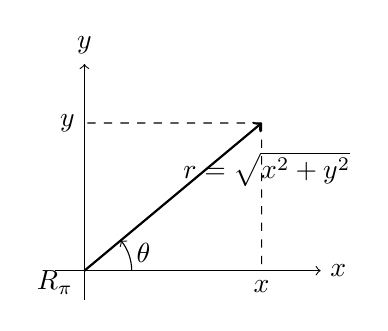
\begin{tikzpicture}[scale=0.75]
            % Axes
            \draw[->] (-0.5,0) -- (4,0) node[right] {$x$};
            \draw[->] (0,-0.5) -- (0,3.5) node[above] {$y$};
            
            % Labels for R^2 and R_+
            \node at (-0.5, -0.2) {$\mathbb{R}_\pi$};
            
            % Point and vector r
            \coordinate (O) at (0,0);
            \coordinate (P) at (3,2.5);
            \draw[->, thick] (O) -- (P) node[midway, above right] {$r = \sqrt{x^2 + y^2}$};
            
            % Dotted lines to the axes
            \draw[dashed] (P) -- (3,0) node[below] {$x$};
            \draw[dashed] (P) -- (0,2.5) node[left] {$y$};
            
            % Angle theta
            \draw[->] (0.8,0) arc[start angle=0,end angle=40,radius=0.8];
            \node at (1,0.3) {$\theta$};
        \end{tikzpicture}
        \end{center}
    \end{minipage}
    \hfill 
    \begin{minipage}{0.45\textwidth}
        \[ \Psi : 
            \begin{cases}
                \R_+^* \times ]0,2\pi[ \rightarrow \R^2 \backslash \R_\pi \\ 
                (r,\theta) \longmapsto (x,y) = (r \cos \theta,r \sin \theta) 
            \end{cases}
        \]
    \end{minipage}

    Alors : 
        \[ J_{\Psi(r,\theta)} =
            \begin{pmatrix}
                \cos \theta & - r \sin \theta \\ 
                \sin \theta & r \cos \theta 
            \end{pmatrix}
        \text{et } |J_{\Psi(r,\theta)}| = r \cos^2 \theta + r \sin^2 \theta = r \in \R_+^* \] 
\end{example}

\begin{corollary}[Passage en polaire]
    Soit $\Psi$ le passage en coordonnées polaires. Alors $\Phi$ est un $C^\infty$-difféomorphisme et 
    pour tout $f \in \overleftarrow{\mathcal{M}_+}(\R^2)$, on a :
        \[  \int_U f(x,y) \;d \lambda_2 = \int_V f(r \cos \theta, r \sin \theta) \times r \; dr d \theta \]
    où $V = \R_+^* \times ]0,2\pi[$
\end{corollary}

\begin{example}[Aire d'un disque]

    Aire d'un disque avec le corollaire fraîchement énoncé :

    \begin{minipage}{0.45\textwidth}
        Soit $A$ l'aire du disque de rayon $R$ centré en $(0,0)$.
        Alors
            \begin{align*}
                A &= \lambda_2(Disque) \\
                &= \int_{\R^2} 1_{Disque}(x,y) \; dxdy
            \end{align*}
    \end{minipage}
    \hfill 
    \begin{minipage}{0.45\textwidth}
        \begin{center}
        \begin{tikzpicture}[scale=0.75]
            % Axes
            \draw[->] (-3,0) -- (3,0) node[right] {$x$};
            \draw[->] (0,-3) -- (0,3) node[above] {$y$};
            
            % Filled Disk
            \filldraw[pattern=north east lines, pattern color=black, draw=black] (0,0) circle (2); % Change 2 to the desired radius
        
            % Label for radius
            \node at (2.5,-0.5) {$r$};
            
            % Center label
            % \node at (0.2, -0.2) {$O$};
        \end{tikzpicture}
        \end{center}
    \end{minipage}
    \begin{align*}
        &= \int_{\R_+^* \times ]0,2\pi[} 1_{Disque}(r \cos \theta, r \sin \theta) \times r \; dr d \theta \\
        &= \int_{0}^{\infty} \Biggl( \int_{0}^{2\pi} 1_{[0,\R[}(r) \times r \; d \theta \Biggr) \; dr \\
        &= \Biggl( \int_{0}^{\infty} 1_{[0,\R[}(r) \times r \; d r \Biggr) \times 2 \pi \\
        &= 2 \pi \int_{0}^{R} r \; dr = 2 \pi \frac{R^2}{2} = \pi R^2 
    \end{align*}
\end{example}

\begin{example}[Gaussienne]
    Soit $\gamma$ la gaussienne sur $\R$ telle que $ \gamma = \int_\R e^{-x^2} \; dx = \sqrt{\pi}$. 
    Vérifions ce résultat. 

    \begin{minipage}{0.45\textwidth}
        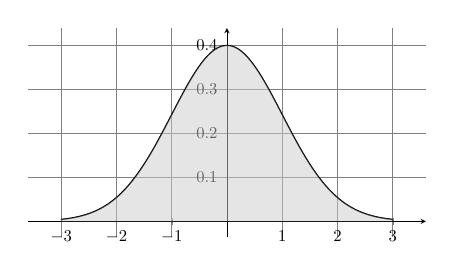
\begin{tikzpicture}[scale=0.6]
            \begin{axis}[
                axis lines = middle,
                grid = both,                 % Fond quadrillé
                grid style={line width=0.5pt, draw=black!50}, % Style des lignes du quadrillage
                xlabel = {},
                ylabel = {},
                domain = -3:3,
                samples = 100,
                width=10cm,
                height=6cm,
                xtick distance=1,            % Distance entre les graduations sur l'axe des x
                ytick distance=0.1,          % Distance entre les graduations sur l'axe des y
                axis line style={black},     % Couleur des axes
                enlarge x limits=0.1,        % Dépassement des axes sur l'axe des x
                enlarge y limits=0.1,        % Dépassement des axes sur l'axe des y
                ]
            \addplot[
                black,                      % Courbe en noir
                thick                       % Épaisseur de la courbe
            ] {exp(-x^2 / 2) / sqrt(2*pi)};
            
            % Dessiner la zone sous la courbe avec un fond gris clair
            \addplot [
                domain=-3:3,
                samples=100,
                fill=black!20,              % Remplissage gris clair
                opacity=0.5,                % Opacité du remplissage
                ] {exp(-x^2 / 2) / sqrt(2*pi)} \closedcycle;
            \end{axis}
        \end{tikzpicture}
    \end{minipage}
    \hfill 
    \begin{minipage}{0.45\textwidth}
        \begin{align*}
            \gamma &= \Biggl( \int_\R e^{-x^2} \; dx \Biggr) \Biggl( \int_\R e^{-y^2} \; dy \Biggr) \\
                    &= \int_\R \Biggl( \int_\R e^{-y^2} \; dy \Biggr) e^{-x^2} \; dx \\
                    &= \int_\R \int_R e^{-x^2-y^2} \; dxdy 
        \end{align*}
    \end{minipage}
    
    \vspace{0.5cm}
    D'après le théorème de Tonelli :
    \[ \int_\R \int_R e^{-x^2-y^2} \; dxdy  = \int_{R^2 \times \R^2} e^{-x^2-y^2} \; dxdy  \] 
    D'après le changement de variable polaire :
    \[ \forall (x,y) \in \R^2 \backslash R_\pi, \quad \exists (x,\theta) \in \R_+^* \times ]0,2\pi[ \text{ tq} \quad (x,y) = (r \cos \theta, r \sin \theta) \]
    D'où : 
    \begin{align*}
        \dots &= \int_{0}^{2\pi} \int_{0}^{\infty} r e^{-r^2 \cos^2 \theta - r^2 \sin^2 \theta} \; dr d\theta \\
            &= \int_{0}^{2\pi} \int_{0}^{\infty} r e^{-r^2} \; dr d \theta = \int_{0}^{2\pi} \Bigl[ - \frac{e^{-r^2}}{2}\Bigr]_0^\infty \; d \theta \\
            &= \int_{0}^{2\pi} \frac{1}{2} \; d \theta = \Bigl[ \frac{1}{2} \theta\Bigr]_0^{2\pi} = \pi 
    \end{align*}
    donc $ \gamma^2 = \pi \Longleftrightarrow \gamma = \pi $
\end{example}

\begin{theorem}[Changement de variable spérique]
    
    \begin{minipage}{0.45\textwidth}
        \[ \Psi :
        \begin{cases}
            \R_+ \times ]-\pi, \pi[ \times ]0,\pi[ \longrightarrow \R^3 \backslash P \\
            (r,\theta,\varphi) \longmapsto     \begin{pmatrix}
                                                x \\
                                                y \\
                                                z 
                                            \end{pmatrix}
            = 
            \begin{pmatrix}
                r \sin \varphi \cos \theta \\
                r \sin \varphi \sin \theta \\
                r \cos \theta
            \end{pmatrix}
        \end{cases}
    \] 
    \begin{align*}
        x &= p \cos \theta = r \sin \varphi \cos \theta \\
        y &= p \sin \theta = r \sin \varphi \sin \theta \\
        z &= r \cos \theta
    \end{align*}
    \end{minipage}
    \hfill 
    \begin{minipage}{0.45\textwidth}
        \begin{center}
            \begin{tikzpicture}[scale=1.25]
                % Points
                \coordinate (origine) at (0,0,0);
                \coordinate (axeX) at (3,0,0);
                \coordinate (axeY) at (0,3,0);
                \coordinate (axeZ) at (0,0,3);
                \coordinate (vecteur) at (2.5,2,2);
    
                % Projections
                \coordinate (projY) at (0,2.5,0);
                \coordinate (projX) at (2.2,0,0);
                \coordinate (projZ) at (0,0,2.7);
                \coordinate (projPlan) at (2.7,0,2.7);
    
                % Dessin des axes
                \draw[->] (origine) -- (axeX) node[right] {$y$};
                \draw[->] (origine) -- (axeY) node[right] {$z$};
                \draw[->] (origine) -- (axeZ) node[right] {$x$};
    
                % Dessin du vecteur
                \draw[->, thick] (origine) -- (vecteur) node[right] {$(x,y,z)$};
    
                % Dessin du vecteur projeté
                \draw[->] (origine) -- (projPlan) node[right] {$p = r \sin \varphi$}; 
    
                % Dessins des projections
                \draw[dotted] (vecteur) -- (projY);
                \draw[dotted] (vecteur) -- (projPlan);
                \draw[dotted] (projPlan) -- (projZ);
                \draw[dotted] (projPlan) -- (projX);
    
                % Dessin des points
                \filldraw (projX) circle (0.5pt);
                \filldraw (projY) circle (0.5pt);
                \filldraw (projZ) circle (0.5pt);
                \filldraw (projPlan) circle (0.5pt);
    
                % Tracer l'angle entre les deux vecteurs
                \draw pic[draw, fill=gray!30, angle radius=1cm, "$\varphi$"] {angle=vecteur--origine--axeY};
                \draw pic[draw, fill=gray!30, angle radius=1cm, "$\theta$"] {angle=axeZ--origine--projPlan};
            \end{tikzpicture}
        \end{center}
    \end{minipage}

    \vspace{0.5cm}

    $\Psi$ est un $C^\infty$-difféomorphisme de Jacobien :
    \[ J_\Psi
        \begin{vmatrix}
            \sin \varphi \cos \theta & - r \sin \varphi \sin \Theta & r \sin \theta \cos \theta \\
            \sin \theta & r \sin \varphi \cos \theta & r \sin \varphi \cos \theta \\
            \cos \theta & 0 & - r \sin \varphi
        \end{vmatrix}
        \dots = r^2 \sin \theta > 0 
    \]
\end{theorem}